\documentclass[12pt,a4paper]{mwart}

\usepackage{lmodern}
\usepackage[T1]{polski}
\usepackage[utf8]{inputenc}

\usepackage[a4paper,
            tmargin=2cm,
            bmargin=2cm,
            lmargin=2cm,
            rmargin=2cm,
            bindingoffset=0cm]{geometry}

\usepackage{tocloft}
\usepackage{hyperref}

\usepackage{amsmath}
\usepackage{amssymb}
\usepackage{siunitx}

\usepackage{graphicx}
\usepackage{subfig}
\usepackage{float}
\usepackage{booktabs}

% Fedora 35 workaround
\pdfmapfile{-mpfonts.map}

\hypersetup{
    colorlinks,
    citecolor=black,
    filecolor=black,
    linkcolor=black,
    urlcolor=black
}

\begin{document}

\title{Wibracje akustyczne warstwy materiału}
\author{Jakub Karbowski}
\date{\today}
\maketitle


\section{Sformułowanie silne}
\begin{align}
    \label{eq:main}
    -\frac{\mathrm{d}^2u}{\mathrm{d}x^2} - u &= \sin x \\
    \label{eq:war1}
    u(0) &= 0 \\
    \label{eq:war2}
    \frac{\mathrm{d}u(2)}{\mathrm{d}x} - u(2) &= 0 \\
    [0,2] \ni x &\to u(x) \in \mathbb{R} \nonumber
\end{align}
Poszukiwana funkcja to $u(x)$.

\section{Sformułowanie słabe}
Równanie \eqref{eq:war1} to zerowy warunek Dirichleta
a~\eqref{eq:war2} to warunek Robina.
Za przestrzeń~$V$ 
przyjmujemy funkcje~$v(x)$ zerujące się na lewym brzegu
$v(0)=0$.
Z~\eqref{eq:war2} dostajemy~$u'(2)=u(2)$.
\begin{align*}
    -u'' - u &= \sin x \\
    -u''v - uv &= v\sin x \\
    \underbrace{-\int_0^2u''v\mathrm{d}x}_\text{przez części} - \int_0^2uv\mathrm{d}x &= \int_0^2v\sin x\mathrm{d}x \\
    -u'v\big|_0^2 + \int_0^2u'v'\mathrm{d}x - \int_0^2uv\mathrm{d}x &= \int_0^2v\sin x\mathrm{d}x \\
    -u'(2)v(2) + u'(0)\underbrace{v(0)}_0 + \int_0^2u'v'\mathrm{d}x - \int_0^2uv\mathrm{d}x &= \int_0^2v\sin x\mathrm{d}x \\
    -\underbrace{u'(2)}_{u(2)}v(2) + \int_0^2u'v'\mathrm{d}x - \int_0^2uv\mathrm{d}x &= \int_0^2v\sin x\mathrm{d}x \\
    \underbrace{-u(2)v(2) + \int_0^2u'v'\mathrm{d}x - \int_0^2uv\mathrm{d}x}_{B(u,v)} &= \underbrace{\int_0^2v\sin x\mathrm{d}x}_{L(v)} \\
\end{align*}
Funkcje $B(u,v)$, $L(v)$ są gotowe do wstawienia do macierzy.

\section{Funkcje bazowe}
Za funkcje bazowe przyjęto
\begin{align*}
    e_i(x) &= \begin{cases}
        \frac{x - x_{i-1}}{x_i - x_{i-1}} & \text{dla $x\in[x_{i-1},x_i]$} \\
        \frac{x_{i+1} - x}{x_{i+1} - x_i} & \text{dla $x\in(x_i,x_{i+1}]$}
    \end{cases} \\
    x_0 &= 0 \\
    x_n &= 2
\end{align*}

\section{Równanie macierzowe}
Usuwamy $e_0$ z macierzy, ze względu na warunek Dirichleta
($u_0 = 0$).
Na prawym brzegu zostaje~$e_n$.
\begin{equation*}
    \left[
    \begin{matrix}
        B(e_1, e_1) & \cdots & B(e_n, e_1) \\
        \vdots      & \ddots & \vdots \\
        B(e_1, e_n) & \cdots & B(e_n, e_n)
    \end{matrix}
    \right]
    \cdot
    \left[
    \begin{matrix}
        u_1 \\
        \vdots \\
        u_n
    \end{matrix}
    \right]
    =
    \left[
    \begin{matrix}
        L(e_1) \\
        \vdots \\
        L(e_n)
    \end{matrix}
    \right]
\end{equation*}

\begin{align*}
    u(x) \approx \tilde{u}(x) = \sum_{i=1}^n\big(u_i \cdot e_i(x)\big)
\end{align*}

\section{Indeksy}
Ponieważ indeksy tablic w~Julii zaczynają się od~1,
$e_0$ we wzorach oznaczane jest przez~$e_1$ w~kodzie.
Należy zwrócić też uwagę na liczbę elementów~$n$.
We wzorach oznacza liczbę elementów, czyli przedziałów.
W~kodzie jest to liczba węzłów = $n+1$.

\section{Program}
Należy pobrać Julię ze strony~\url{https://julialang.org}.
Testowane na wersji~1.7.1, spokojnie powinno działać na~>1.5.0.
Program można włączyć komendą:
\begin{verbatim}
julia src/main.jl
\end{verbatim}
Po obliczeniach pokaże się okno z~wykresem.
Plik~\verb|src/main.jl| jest tylko skryptem
uruchamiającym.
Główny algorytm jest w~pliku~\verb|src/rurki.jl|.
Pierwsze obliczenia będą wolne, ze względu
na kompilator JIT. Potem już śmiga
(u mnie $N=5000$ jeszcze policzy, dalej trzeba poczekać).

\begin{figure}[h]
    \centering
    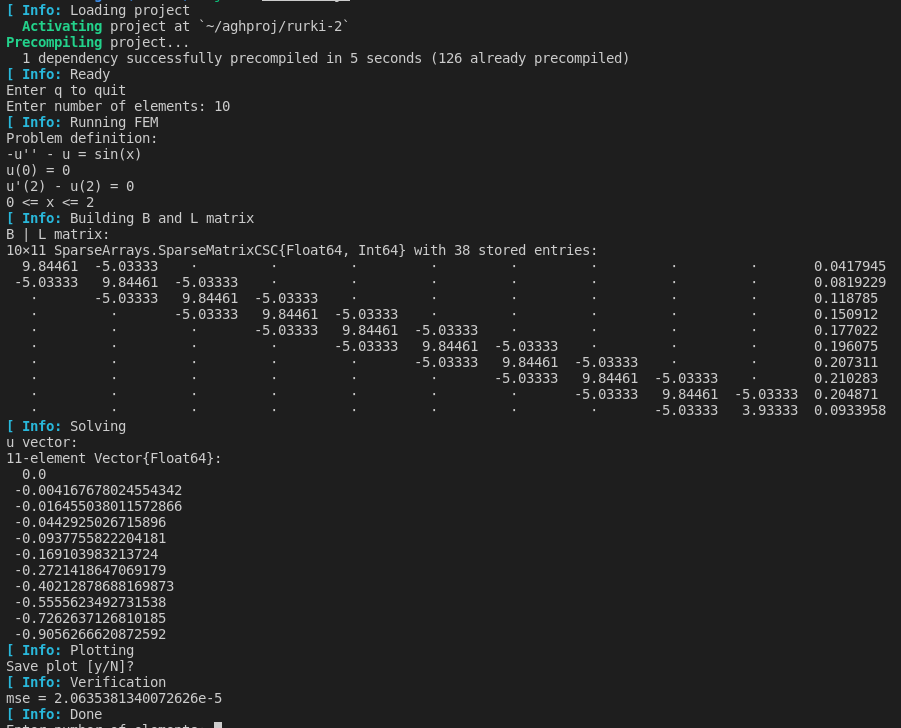
\includegraphics[width=\textwidth]{images/rurki-log.png}
    \caption{Przykładowe uruchomienie programu}
    \label{rys:rurki-log}
\end{figure}

\section{Wyniki}
Rozwiązanie analityczne to
\begin{equation*}
    \frac{1}{2} \left(x\cos{x} + \frac{\sin(x) (2\sin{2} + \cos{2})}{\cos{2} - \sin{2}}\right)
\end{equation*}
Na wykresie Rys.~\ref{rys:rurki-n3} ,,widać'', że się zgadza.
Dodatkowo obliczono \textit{mean squared error}
dla 40~punktów ($N=3$). $\text{mse} = 0.00026$.
\begin{figure}[h]
    \centering
    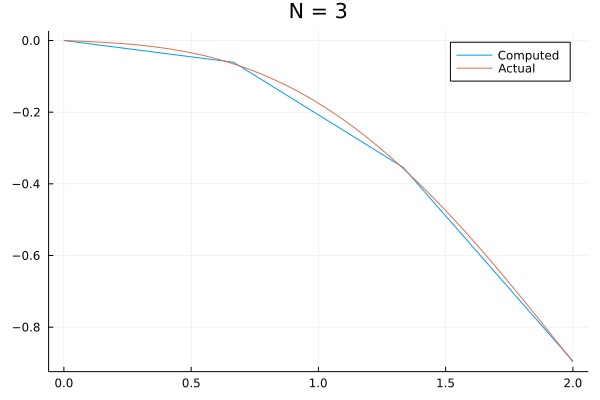
\includegraphics[width=0.8\textwidth]{images/rurki-n3.png}
    \caption{Wyniki dla $N=3$}
    \label{rys:rurki-n3}
\end{figure}


\end{document}